% The original template for ICIP-2000 paper; to be used with:
%          spconf.sty  - ICASSP/ICIP LaTeX style file, and
%          IEEEbib.bst - IEEE bibliography style file.
% --------------------------------------------------------------------------
\documentclass{article}
\usepackage{spconf,amsmath,epsfig,url}
\usepackage[section]{placeins}

% Example definitions.
% --------------------
\def\x{{\mathbf x}}
\def\L{{\cal L}}

% Title.
% ------
\title{stock Price Prediction}
%
% Single address.
% ---------------
\name{Thanit Tativannarat, Phathit Sriburi, Nattanat Chatthee, Natthanon Tunyanun}


\address{Department of Computer Engineering\\ Chulalongkorn Univerisy\\ Bangkok, Thailand}

% For example:
% ------------
%\address{School\\
%		 Department\\
%		 Address}
%
% Two addresses (uncomment and modify for two-address case).
% ----------------------------------------------------------

\begin{document}
%\ninept
%
\maketitle
%
\begin{abstract}
Predicting a stock price is a very challenge task.It requires high accuracy go together with high flexibility.Nowadays, there are many people working about Algorithmic trading.May be this is the new trend or it can be a new job that appeared in the future. 
\end{abstract}

\section{Introduction}\label{sec:intro}

\subsection{Motivation}

Nowaday, we can see many of securities company provide a software that help customers to plan their investment strategy.
the software is also known as EA (Expert Advisor) ,this brings our team curiosity.Does the EA really work? Our target is to analyze the models and to find out which model is the most practical in the stock market.

\subsection{Previous Work}
There are many different works about predicting stock price. Some of them use linear regression model,Long Short Term Memory (LSTM),Gated Recurrent Unit (GRU),Recurrent Neural Network (RNN) to deal with time series data.Some of them use Convolutional Neural Network (CNN) to find the chart pattern in the stock chart.

\subsection{What We Are Going to Do}

Before our experiments, we tried some basic Deep Neural Network that base on dataset without feature engineering and found that the test score is not good as we expected.After that, our team tried to add some useful features such as moving average to the dataset but, the test score of our new model stills not good as we expected.We found that we did not deal with noises in the dataset.The noise can be generated by trading psychology or news.These leads to focusing on the noises.After that,we create the ARIMA model that relate with time-series data.The result of the model still like the others.\\We know that Newyork stock market (Dowjones) opened before Japan stock market (Nikkei) and these two stock markets are not overlapse each other.Our next milestone is using the close price of Dowjones stock market to predict the close price of Nikkei stock market.

\subsection{Organization of the Paper}

In Section Necessary Background we provide the background on the investment, basic time-series analysis, Machine Learning and Backtesting.



\section{Necessary Background}
\label{sec:background}


We divide topics in this part into 6 parts are as follows :\\
1. Knowledge about investment\\
2. What is time-series\\
3. ARIMA model\\
4. Feature engineering\\
5. Training a model\\
6. Backtesting\\


\subsection{Investment}
Everyday,there are many investors trade stocks with each other.The buyers have the money but, they would like to hold stocks instead of money , on the other hand , the sellers already have stocks but, they would like to sell their stocks and keep money instead.The market is the place that allow investors to trade with each other.Trading transaction will be happened when buyer and seller make a deal.
Price mechanism is also created by this event too.

\subsection{Basic time-series Analysis}
\begin{itemize}
\item What is time-series?\\A time series is a sequence of data that ordered by time.Stock price at time N will 
effect to stock price at time N+1
\item Stocks data is also a time series that has seasonality (each stock has opportunity day itself).
\end{itemize}


\subsection{ARIMA Model}
ARIMA, short for "Auto Regressive Integrated Moving Average", is one of the machine learning model for manipulate with time series data.The ARIMA model is divided into 3 terms :\\p is the order of AR term\\q is the order of MA term\\d is the number of differencing required to make the time series stationary.\\This model is very flexible and has strong underlying theory.Main concepts of this model are about order and differencing of the dataset. 

\subsection{Feature engineering}
Feature engineering is the method that add some useful data to the dataset.This method is created for improving the model.

\subsection{Model training}
Model training is how to make a model learns from data that feeded into it.The model will improve itself by tuning the hyperparameters to minimize loss.

\subsection{Backtesting}
Backtesting is the process that use the model to predict the output then, display or find errors between the output and the test data.This process is for testing how much flexibility does the model have. 

\section{Your Proposed Method}\label{sec:yourmethod}
This section is about feature engineering and implementation's details.

\subsection{Dataset}
First, download these two dataset from link below.All dataset which is used in our experiment are from Yahoo Finance.

\begin{itemize}
\item Dowjones dataset\\
\url{https://finance.yahoo.com/quote/%5EDJI/history?p=%5EDJI}
\\Enter Time Period as you like, Choose Frequency to Daily then Press Download Data button.
\end{itemize}

\begin{itemize}
\item Nikkei dataset\\
\url{https://finance.yahoo.com/quote/%5EN225/history?p=%5EN225}
\\Enter Time Period as you like, Choose Frequency to Daily then Press Download Data button.
\end{itemize}

When your download is finished, you would receive a CSV file that contains basic market data (open price, high, low, close price and volume).


\subsection{Feature engineering}
After the previous part,Our team join two CSV files together by appending Nikkei dataset at day N to Dowjones dataset at day N-1 for nikkei combine with dowjones V1 model and nikkei combine with dowjones V2 model.

\subsection{Design of the model}
We created three models that have different layers design.\\

1. nikkei without feature engineering\\

\label{sec:latex}
\begin{figure}
  \centering
  \centerline{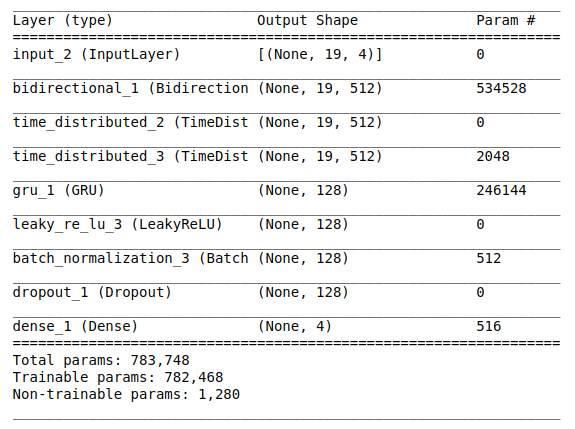
\includegraphics[width=0.45\textwidth]{nk_n_fe.png}}
  \caption{nikkei without feature engineering}
  \label{fig:bibtex}
\end{figure}

2. nikkei combine with dowjones V1\\

\label{sec:latex}
\begin{figure}
  \centering
  \centerline{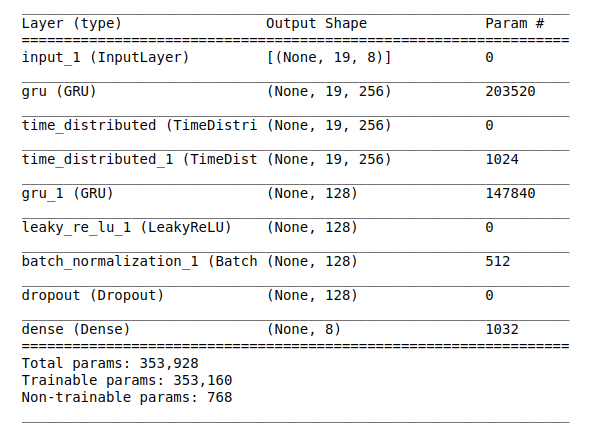
\includegraphics[width=0.45\textwidth]{V1.png}}
  \caption{nikkei combine with dowjones V1}
  \label{fig:bibtex}
\end{figure}

3. nikkei combine with dowjones V2 (Bidirectional)\\

\label{sec:latex}
\begin{figure}
  \centering
  \centerline{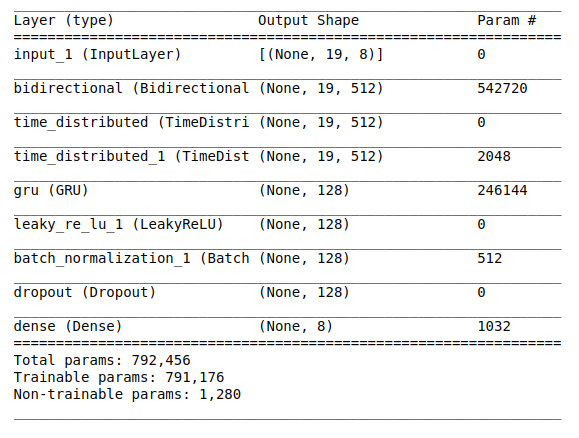
\includegraphics[width=0.45\textwidth]{V2.png}}
  \caption{nikkei combine with dowjones V2}
  \label{fig:bibtex}
\end{figure}


\subsection{Model training}
First, we use factor=0.8, patience=4, min lr=0.0001, batch size=64,epochs=300 and optimizer Adam(0.005)  for nikkei without feature engineering model.\\Second, we use factor=0.9, patience=3, min lr=1e-9, batch size=1000, epochs=500 and Adam(lr=1e-2, decay=1e-2) for nikkei combine with dowjones V1 model.\\Last model, we use factor=0.9, patience=3, min lr=1e-9, batch size=1000, epochs=500 and Adam(lr=1e-5, decay=1e-4) for nikkei combine with dowjones V2 model.



\section{Experimental Results}
Testing method for time series data has two ways\\

1. Expanded window\\

This method is used for testing the data in the past.\\

2. Sliding window\\

This method is used for tesing new data.\\



\label{sec:exp}
\label{sec:latex}
\begin{figure}
  \centering
  \centerline{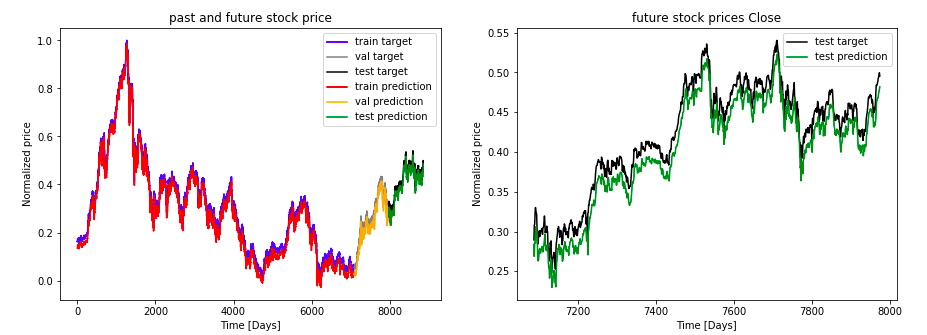
\includegraphics[width=0.45\textwidth]{test1.png}}
  \caption{Backtesting nikkei without feature engineering model by expanded window and sliding window}
  \label{fig:bibtex}
\end{figure}

\label{sec:latex}
\begin{figure}
  \centering
  \centerline{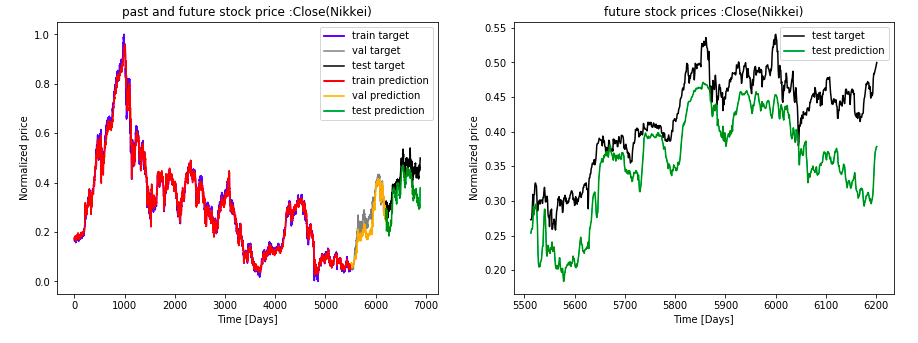
\includegraphics[width=0.45\textwidth]{test2.png}}
  \caption{Backtesting nikkei combine with dowjones V1 model by expanded window and sliding window}
  \label{fig:bibtex}
\end{figure}

\label{sec:latex}
\begin{figure}
  \centering
  \centerline{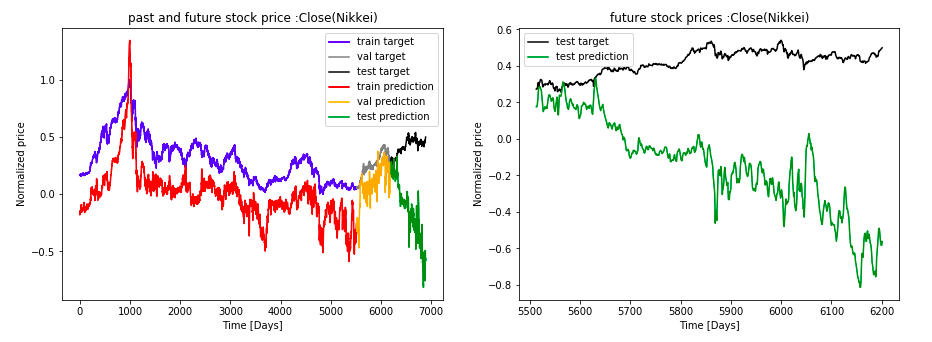
\includegraphics[width=0.45\textwidth]{test3.png}}
  \caption{Backtesting nikkei combine with dowjones V2 model by expanded window and sliding window}
  \label{fig:bibtex}
\end{figure}

\begin{table}
\centering
\begin{tabular}{|l|c|c|c|c|} % this defines how many columns and indentation of each column
 \hline % creates a horizontal line
Models & train & test & validate \\ %columns are separated by & and newline is \\
 \hline
 nikkei without feature engineering & 0.00064 & 0.00049 & 0.00068 \\
 nikkei combine with dowjones V1 & 0.00030 & 0.07512 & 0.01022 \\
 nikkei combine with dowjones V2 & 0.08058 & 12.39508 & 0.78669 \\
\hline
\end{tabular}
\caption{Loss of the model}
\label{tab:table}
\end{table}


\section{Conclusions}
\label{sec:conclusion}
Every markets has it own flactuation.When we try to combine the data of both markets and the data is not denoised before model training, the created model is worse than the nikkei without feature engineering model.So, the nikkei without feature engineering model has the best result.In the real world, EA can be created by using machine learning model or rule-based programming but now, rule-based programming still better than machine learning model because of many reasons such as the number of data or knowledge about data.



% References should be produced using the bibtex program from suitable
% BiBTeX files (here: bibl_conf). The IEEEbib.bst bibliography
% style file from IEEE produces unsorted bibliography list.
% -------------------------------------------------------------------------
\bibliographystyle{IEEEbib}
\bibliography{conference}

\end{document}

